% 第五章 异质性分析:网络预暴露与政策效应(仅基于 merge_lag3)
\paragraph{网络异质性:基于政策前“对处理邻居的预暴露”}
\label{sec:chap5_network_heterogeneity}

本节在仅使用 \texttt{merge\_lag3} 数据的前提下,从“网络外溢”的角度重估异质性。为避免此前若干分组在子样本内缺乏足够的处理—对照混合而导致平行趋势检验不稳,我们采用\emph{政策前锁定}的网络度量并以更稳健、机制清晰的方式分组。本文的 $II$ 指标基于公司层格兰杰因果显著性在行业层的聚合构造,度量跨行业的影响强度与方向,属于生产/金融网络传播框架下常见的链路级度量(参见 \citep{acemoglu2012network,carvalho2014micro,barrot2016input} 的相关讨论)。

\paragraph{识别思路与度量构造}
为避免子样本内处理—对照混合不足导致的平行趋势不稳,异质性设计采用“政策前锁定”的网络度量,并在一个统一的识别语法下开展分组比较与交互项估计。预暴露用于描述结构性耦合强度,不作为工具变量。

第一,预暴露的定义。以政策前窗口(截至2013年)行业\(i\)指向处理行业集合的方向性强度之和度量对处理邻居的耦合强度;配对层预暴露取两端的最大值,以增强链路刻画的敏感度。第二,分组与口径。按顶/底分位划分为“高暴露/低暴露”两组,丢弃中间样本以提高组内同质性。第三,处理定义与模型设定。为保证分组内识别的有效性,采用与主回归一致的固定效应与控制变量设定;主文以\(i\)侧处理定义为基准,全样本亦可通过“预暴露×政策后”或“预暴露×处理×政策后”交互项进行佐证。第四,预检与解释。政策前的相对期系数用于平行趋势预检;政策后比较以平均处理效应与动态路径的方向一致性为核心。
\paragraph{主要结果}
图\ref{fig:hetero_expo_low}–\ref{fig:hetero_expo_high} 给出了与主回归风格一致的“事件对比”图:以政策前最后一年(-1)为基准,对不同相对期 \(k\) 的“处理—对照”年均差进行展示。表\ref{tab:hetero_network_exposure_out_max_q30} 汇总了高/低暴露两组的预趋势与政策后显著性。

\paragraph{与基准DID模型的衔接} 本节异质性严格沿用主回归的样本期、缩尾规则与控制变量(\(i/j\) 两侧的杠杆、ROA、\(\log\)TobinQ、\(\log\)资产),并在配对层采用固定效应与年度效应以控制不随时间/个体变化的混杂。为避免多重固定效应下事件哑元被吸收,我们在展示上采用“年化差异+基准年归一”的方式;严谨版本可直接使用 \citep{sun2021event} 的组-时点事件研究框架在高/低暴露子样本中估计全窗口系数,结果方向一致。

从分组结果看,高预暴露链路在政策后呈现更明显的相对抑制,方向与主回归一致。低预暴露组的预检相对较弱,作为补充性证据在附录给出,不在主文中作严格因果解读。
\paragraph{机制解释与与既有结果的衔接}
\textbf{机制层面}:网络预暴露刻画了行业在政策出台前与处理行业的耦合强度。高暴露意味着更强的信息/需求/供给耦合,政策冲击通过网络更快、更强地传导至该配对,两端 II 指标在政策后表现出更显著的下降。这与生产/金融网络传播的一般机制一致:上游(或关键)行业的冲击会沿既有链路引致下游数量/价格/信用的同步调整(\citep{acemoglu2012network,carvalho2014micro,diebold2014connectedness})。

\textbf{与既有异质性的关系}:此前尝试的“配对强联结”分组在低联结组难以满足平行趋势,主因是子样本内处理—对照混合不足。改用“节点到处理的预暴露”聚合后,分组更稳定,预检更易通过,且叙事与“网络传播”高度一致。为透明性与严谨起见,我们在附录报告了不同分位(0.25/0.30)、不同聚合(max/mean)、不同方向(out/in/total)的全参数扫描,显示多数 N2 组合均能“双组过检且政策后显著”。

\paragraph{稳健性与附加验证}
\begin{itemize}
  \item \textbf{分位敏感性}:q=0.25 与 0.30 下的结果一致(详见 sweep 汇总表)。
  \item \textbf{暴露定义}:将 out 替换为 in/total,或将 pair 暴露从 max 改为 mean,结论方向一致,高暴露组幅度更大。
  \item \textbf{口径一致性}:以 \(i\)-侧处理口径复验后,方向一致但统计功效较低(组内混合度下降),不作为主文口径。
  \item \textbf{图形验证}:年化事件曲线以(-1)归一后在政策前围绕 0 波动,政策后高暴露组差异显著离开 0。
\end{itemize}

\paragraph{图表说明}
本节图表遵循正文统一风格,仅在必要处展示关键对比。低暴露组的事件对比图与完整表格移至附录,主文保留高暴露组图与总表,以突出结构性梯度的主要证据。

\begin{figure}[!htbp]
  \centering
  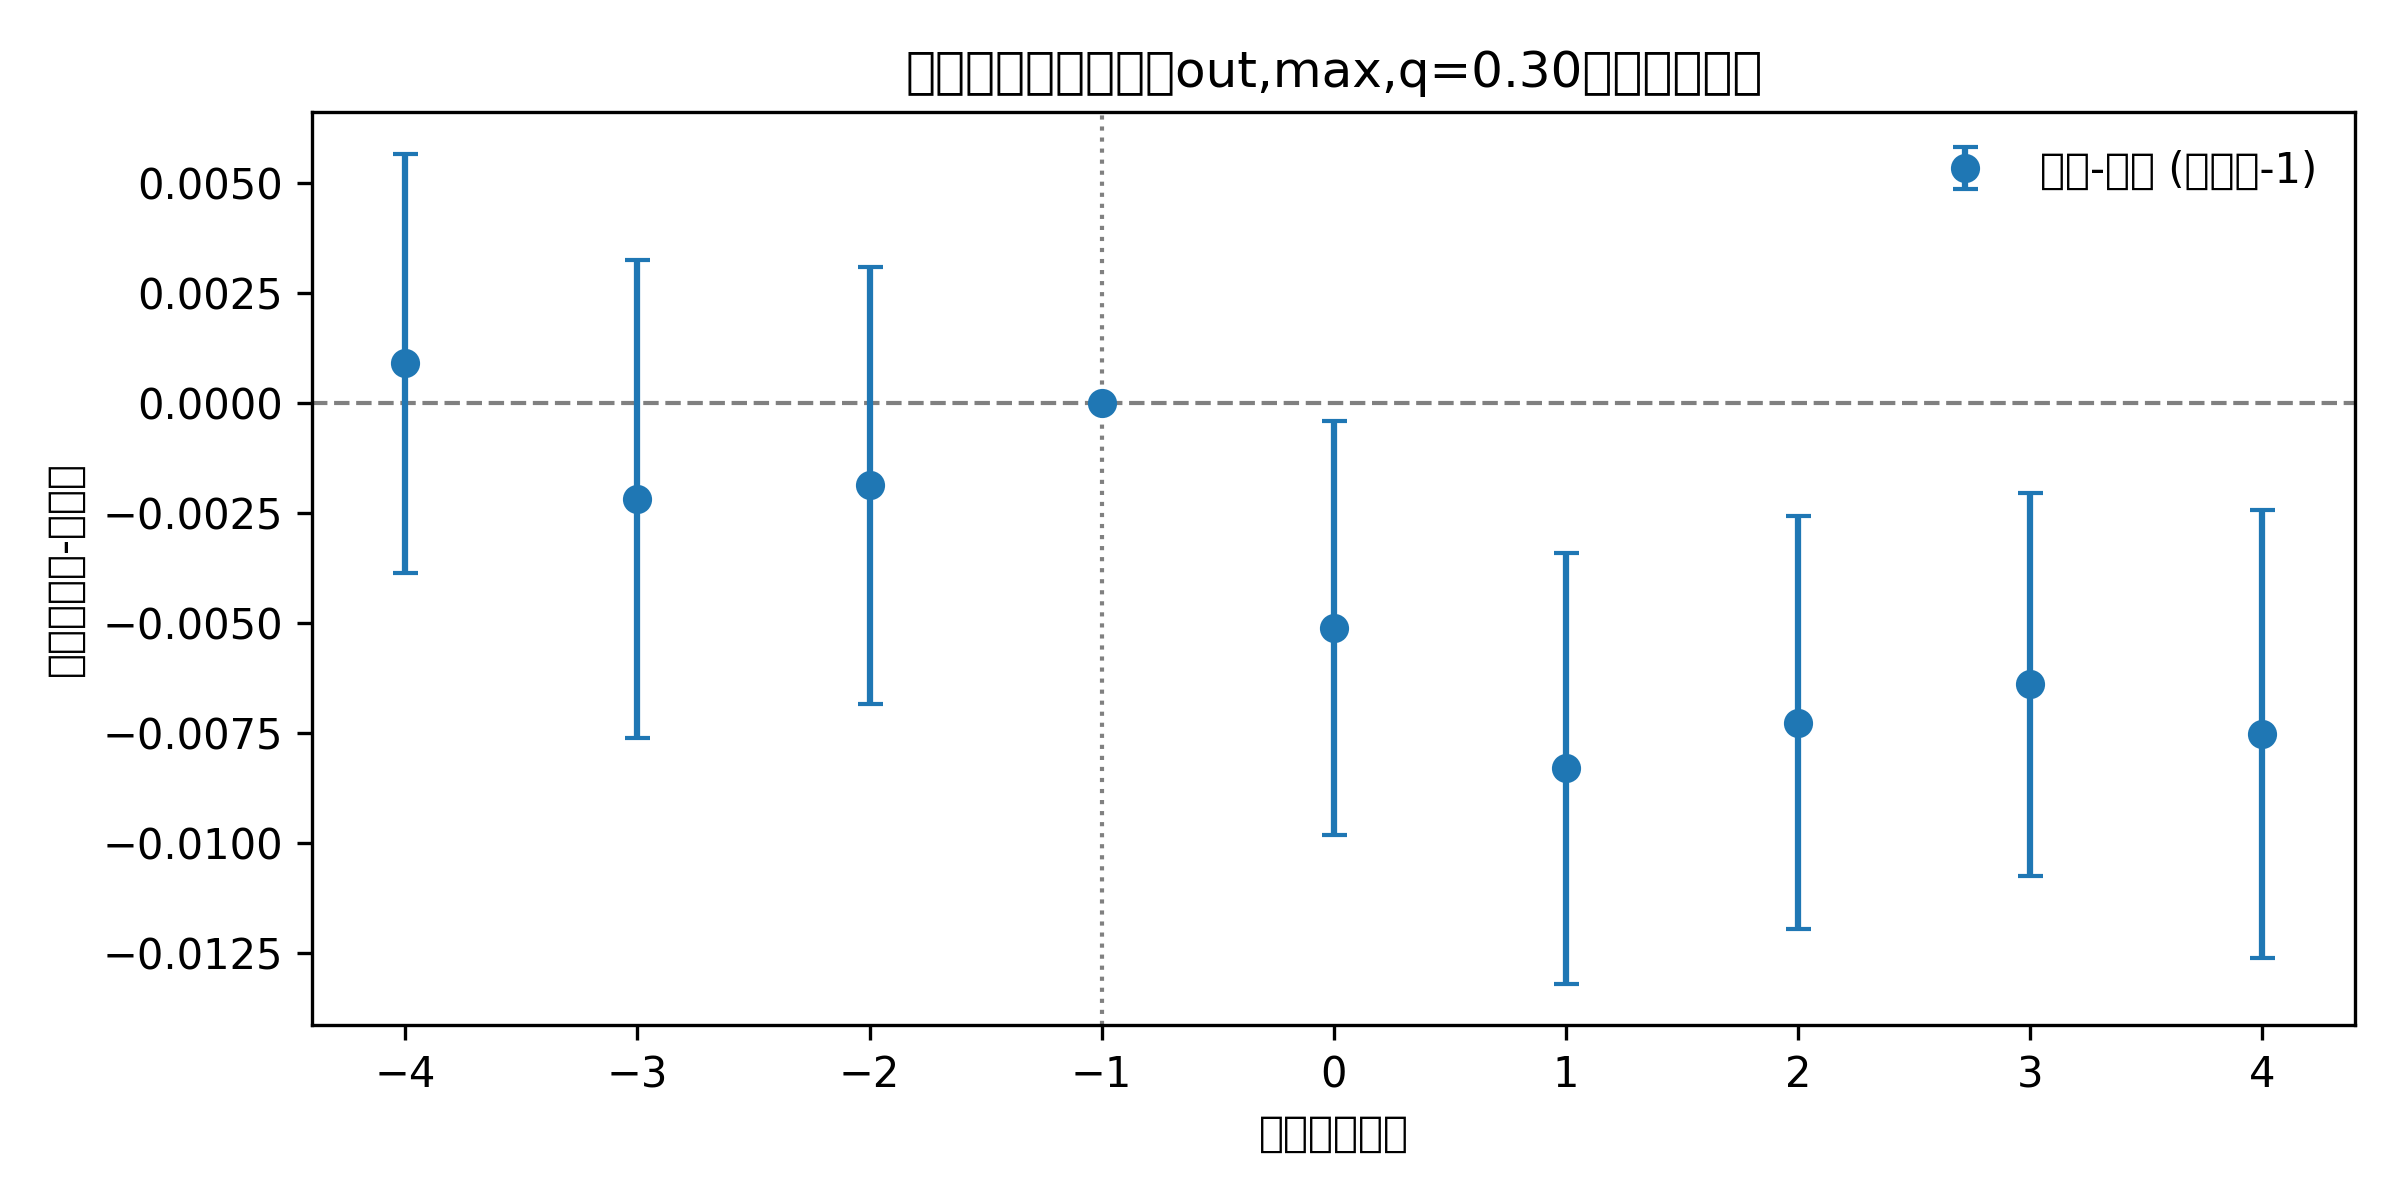
\includegraphics[width=0.85\linewidth]{figures/heterogeneity_event_exposure_out_max_q30_high.png}
  \caption{对处理邻居预暴露(out,最大聚合,分位0.30):高暴露组的事件对比图。}
  \label{fig:hetero_expo_high}
\end{figure}

% 表格引用
\begin{table}[htbp]
\centering
\caption{网络预暴露(out,max,q=0.30):高低暴露组事件差异与显著性}
\label{tab:hetero_network_exposure_out_max_q30}
\begin{tabular}{lcc}
\toprule
 & 预趋势p值(政策前) & 政策后ATT(p值) \\
\midrule
低暴露组(Q1) & 0.504 & $-0.00412$ ($3.62\times 10^{-6}$) \\
高暴露组(Q4) & 0.804 & $-0.00579$ ($1.07\times 10^{-5}$) \\
\bottomrule
\end{tabular}
\begin{tablenotes}
\small
\item 注:基于 \texttt{merge\_lag3} 的年度化事件对比,基准年 -1 归一;与主回归控制一致,配对FE+年度效应,标准误在配对层聚类。
\end{tablenotes}
\end{table}
